\documentclass[10pt]{article}
\usepackage[utf8]{inputenc}
\usepackage[swedish]{babel}

\def\ordf{Daniel Bakic}
\def\sekr{Axel Voss}
\def\fvc{Magnus Lundh}

\def\doctype{Handlingar} %ex. Kallelse, Handlingar, Protkoll
\def\mname{Höstterminsmötet} %ex. styrelsemöte, vårterminsmöte
\def\mnum{HT/18} %ex S02/16, E01/15, VT/13
\def\date{2018-11-22} %YYYY-MM-DD
\def\docauthor{\sekr}
 
\def\mtime{17:15}
\def\place{E:A}

\usepackage{../../_sektion-handlingar/e-handlingar-sek}
\usepackage{../../e-mote}
\usepackage{../../../../e-sek}

\begin{document}

\firstpage{{\doctype} till {\mname} {\mnum}}{{\date} {\mtime} i {\place}}

\tableofcontents
\newpage

\subfile{../../_sektion-handlingar/_other/guide}
\newpage

\section{Dagordning}
\subsection{Tid och plats}
\tidplats

\subsection{Föredragningslista}
\begin{paralist}
	\pli{TaFMÖ}{}
	\pli{Val av mötesordförande}{}
	\pli{Val av mötessekreterare}{}
	\pli{Godkännande av tid och sätt}{}
	\pli{Val av två justeringspersoner}{}
	\pli{Adjungeringar}{}
	\pli{Godkännande av dagordningen}{}
	\pli{Föregående sektionsmötesprotokoll}{}
	\pli{Meddelanden}{}
	\pli{Beslutsuppföljning}{}
	\pli{Utskottsrapporter}{}
	\pli{Uppföljning av verksamhetsplan}{}
	\pli{Ekonomisk rapport}{}
	\pli{Uttag ur Sektionens fonder sedan förra terminsmötet}{}
	\pli{Resultatrapport från första halvan av verksamhetsåret}{}

	\pli{Behandling av motioner}{}
	\begin{paralist}
		\pli{StraffBong}{}
		\pli{Hotell Brödraskapet}{}
		\pli{Sektionsgrodan}{}
		\pli{Uppgradera utrustning i Edekvatas kök}{}
		\pli{Kuddar i Diplomat}{}
		\pli{Ändring av hur sektionen väljer NollU-funktionärer}{}
		\pli{Uppdatering av postbeskrivning för Övergudphadder}{}
		\pli{Ta bort NollU:s representant i valberedningen}{}
		\pli{Suppleant för Øverphøs}{}
		\pli{Ändringar för val av Øverphøs och Co-phøs}{}
		\pli{Wiki}{}
	\end{paralist}
	\pli{Behandling av propositioner}{}
	\begin{paralist}
		\pli{Budgetförslag för 2019}{}
		\pli{Verksamhetsplansförslag för 2019}{}
		\pli{Flytta HTF-ansvariga till SRE}{}
		\pli{Uppdatering av policy för nycklar och access}{}
		\pli{Uppdatering av policy Principer för deltagande i Sektionsaktiviteter}{}
		\pli{Uppdatering av policy för Inbjudningar och anmodningar}{}
		\pli{Inköp av toppar till Vega}{}
	\end{paralist}
	\pli{Övrigt}{}
	\pli{TaFMA}{}
\end{paralist}

\begin{signatures}{2}
	\emph{I Sektionens tjänst}
	\signature{\ordf}{Ordförande}
	\signature{\sekr}{Kontaktor}
\end{signatures}

\subfile{../_other/ekonomisk_rapport}
\newpage
\addcontentsline{toc}{subsection}{Balansrapport}
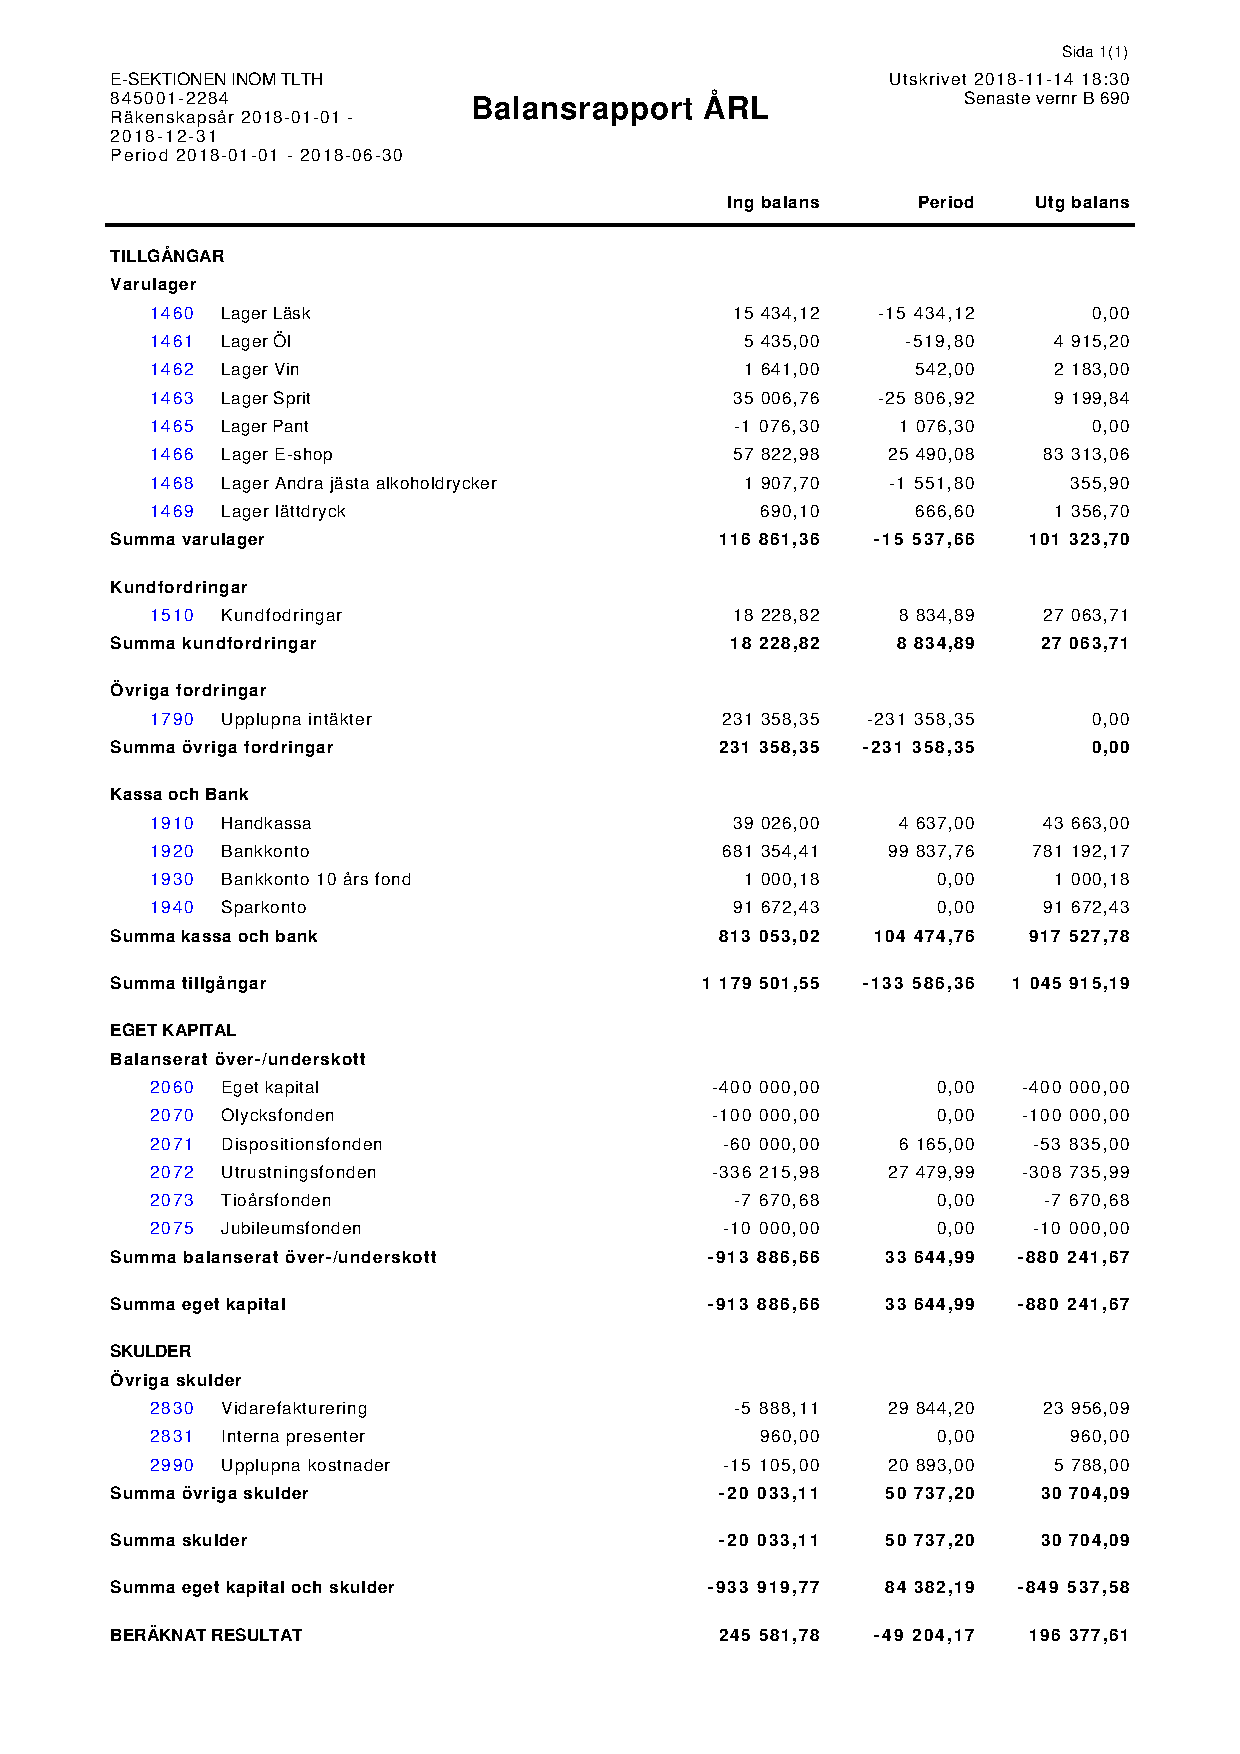
\includepdf[pages=1]{../_res/balansrapport.pdf}


\subfile{../_other/uttag}
\newpage

\begin{supersection}{Beslutsuppföljningar}{}
	\subsection{Överblick}
	\begin{busek}
		\beslutsek{HT/17}{Veckoliga studiekvällar med tilltugg}{William Marnfeldt, Filip Larsson}{}{} %kolla upp!!
		\beslutsek{VT/18}{Uppdaterad utrustning för linbanan}{Jonatan Kronander, Filip Kronström, Magnus Lundh}{Inköp av nytt material till linbanan för en kostnad av \SI{1500}{kr}}{HT/18}
		\beslutsek{VT/18}{Inköp av en ny sektionskamera}{Eltayeb Bayomi}{}{HT/18}
		\beslutsek{VT/18}{Utskottstack i form av märken}{Henrik Ramström}{}{HT/18}
		\beslutsek{VT/18}{Inköp Umphbox}{Styrelsen 2018}{}{HT/18}
		\beslutsek{VT/18}{Mikrovågsugnar}{Styrelsen 2018}{}{HT/18}
	\end{busek}

	\newpage
	\subfile{../besuppf/studie}
	\subfile{../besuppf/als}
	\subfile{../besuppf/kamera}
	\subfile{../besuppf/tack}
	\subfile{../besuppf/umph}
	\subfile{../besuppf/micro}
\end{supersection}

\begin{utskottsrapporter}
	\subfile{../utskottsrapporter/cm}
	\subfile{../utskottsrapporter/e6}
	\subfile{../utskottsrapporter/enu}
	\subfile{../utskottsrapporter/fvu}
	\subfile{../utskottsrapporter/infu}
	\subfile{../utskottsrapporter/km}
	\subfile{../utskottsrapporter/noju}
	\subfile{../utskottsrapporter/nollu}
	\subfile{../utskottsrapporter/sre}
	\subfile{../utskottsrapporter/styrelsen}
	\subfile{../utskottsrapporter/vb}
\end{utskottsrapporter}

\begin{supersection}{Verksamhetsplaner}{}
	\subfile{../verksplaner/2018}
\end{supersection}

\begin{supersection}{Uppföljningar av verksamhetsplaner}{}
	\subfile{../verksplanuppfar/2018-vt}
	\subfile{../verksplanuppfar/2018-ht}
\end{supersection}

\begin{motioner}
	\subfile{../motioner/bong}
	\subfile{../motionssvar/bong}

	\subfile{../motioner/brodrarskap}
	\subfile{../motionssvar/brodrarskap}

	\subfile{../motioner/groda}
	\subfile{../motionssvar/groda}

	\subfile{../motioner/kok}
	\subfile{../motionssvar/kok}

	\subfile{../motioner/kuddar}
	\subfile{../motionssvar/kuddar}

	\subfile{../motioner/nollu}
	\subfile{../motionssvar/nollu}

	\subfile{../motioner/ogp}
	\subfile{../motionssvar/ogp}

	\subfile{../motioner/repvb}
	\subfile{../motionssvar/repvb}

	\subfile{../motioner/suppleant}
	\subfile{../motionssvar/suppleant}

	\subfile{../motioner/val}
	\subfile{../motionssvar/val}

	\subfile{../motioner/wiki}
	\subfile{../motionssvar/wiki}
\end{motioner}

\begin{propositioner}
	\subfile{../propositioner/_budget}
	\subfile{../propositioner/_verkplan}

	\subfile{../propositioner/htf}
	\subfile{../propositioner/access}
	\subfile{../propositioner/aktiviteter}
	\subfile{../propositioner/inbjudningar}
	\subfile{../propositioner/toppar}
\end{propositioner}

\begin{supersection}{Halvårsbokslut 2018}{}
	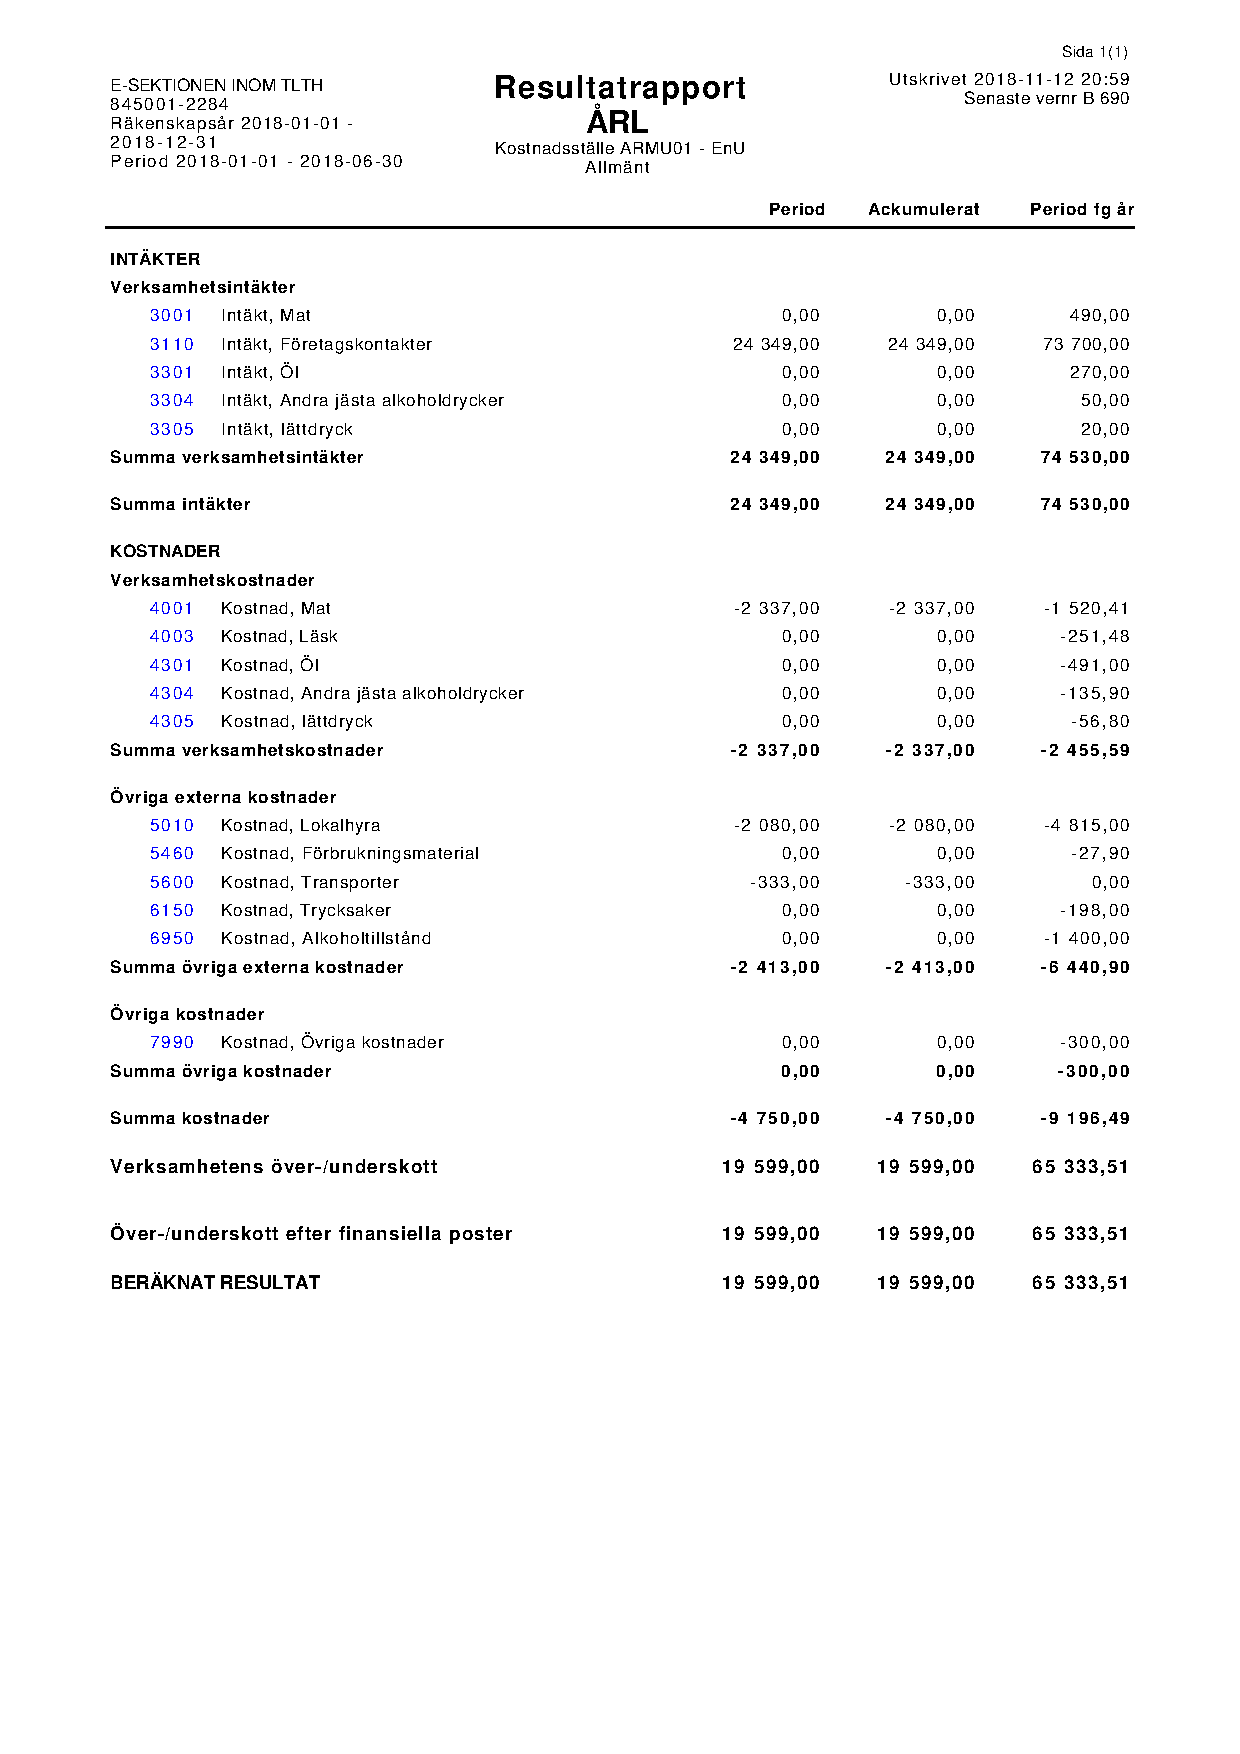
\includepdf[pages=-]{../_res/resultatrapport.pdf}
\end{supersection}

\end{document}
